\section{Divergence-free FE space}
\label{sec:divFreeSpace}
The divergence-free constraint of the magnetic field, $\nabla \cdot \bfB = 0$ (Gauss's law) is not enforced by the solution definition in \cref{weakSlnDef}. Therefore, we need to perform additional work to be sure that we do not have a non-physical solution in the sense that the constraint is not satisfied.
\paragraph{}
There are two often used approaches to handle this problem - the Constraint-Transport (CT) method, and divergence cleaning. The first one is not suitable for this work, as it constraints the triangulation in such a way, that implementing Adaptive Mesh Refinement would be very complicated, if possible at all. The second approach, the divergence cleaning methods need additional postprocessing step which may be omitted for the sake of calculation efficiency. The approach taken in this work is to replace the standard FE space  \cref{feSpaceDef} with basis functions \cref{feSpaceBasis} for the magnetic field part ($B$) with a vector-valued (3-dimensional) space $V_h^B$ of functions that have exactly
\be
\nabla \cdot \mrvh^B = 0,\ \ \mrvh^B\in V_h^B,
\ee
where these functions are as before discontinuous on interfaces $\Gamma_{ij}$.
The basis of space $V_h^B$ for piecewise-linear functions can be selected in several ways, in this work, the following basis was selected:
\begin{table}[H]
	\begin{tabular*}{\textwidth}{cccc}
		\hline\\
		$\lo\begin{array}{c}B_x\lo x, y, z\ro\\B_y\lo x, y, z\ro\\B_z\lo x, y, z\ro \end{array}\ro$ & Visualization & $\lo\begin{array}{c}B_x\lo x, y, z\ro\\B_y\lo x, y, z\ro\\B_z\lo x, y, z\ro \end{array}\ro$ & Visualization \\ 
		\\ \hline
	\end{tabular*}
	\\
	\begin{tabular*}{\textwidth}{cccc}
		$\lo\begin{array}{c}1\\0\\0 \end{array}\ro$ & \raisebox{-0.5\totalheight}{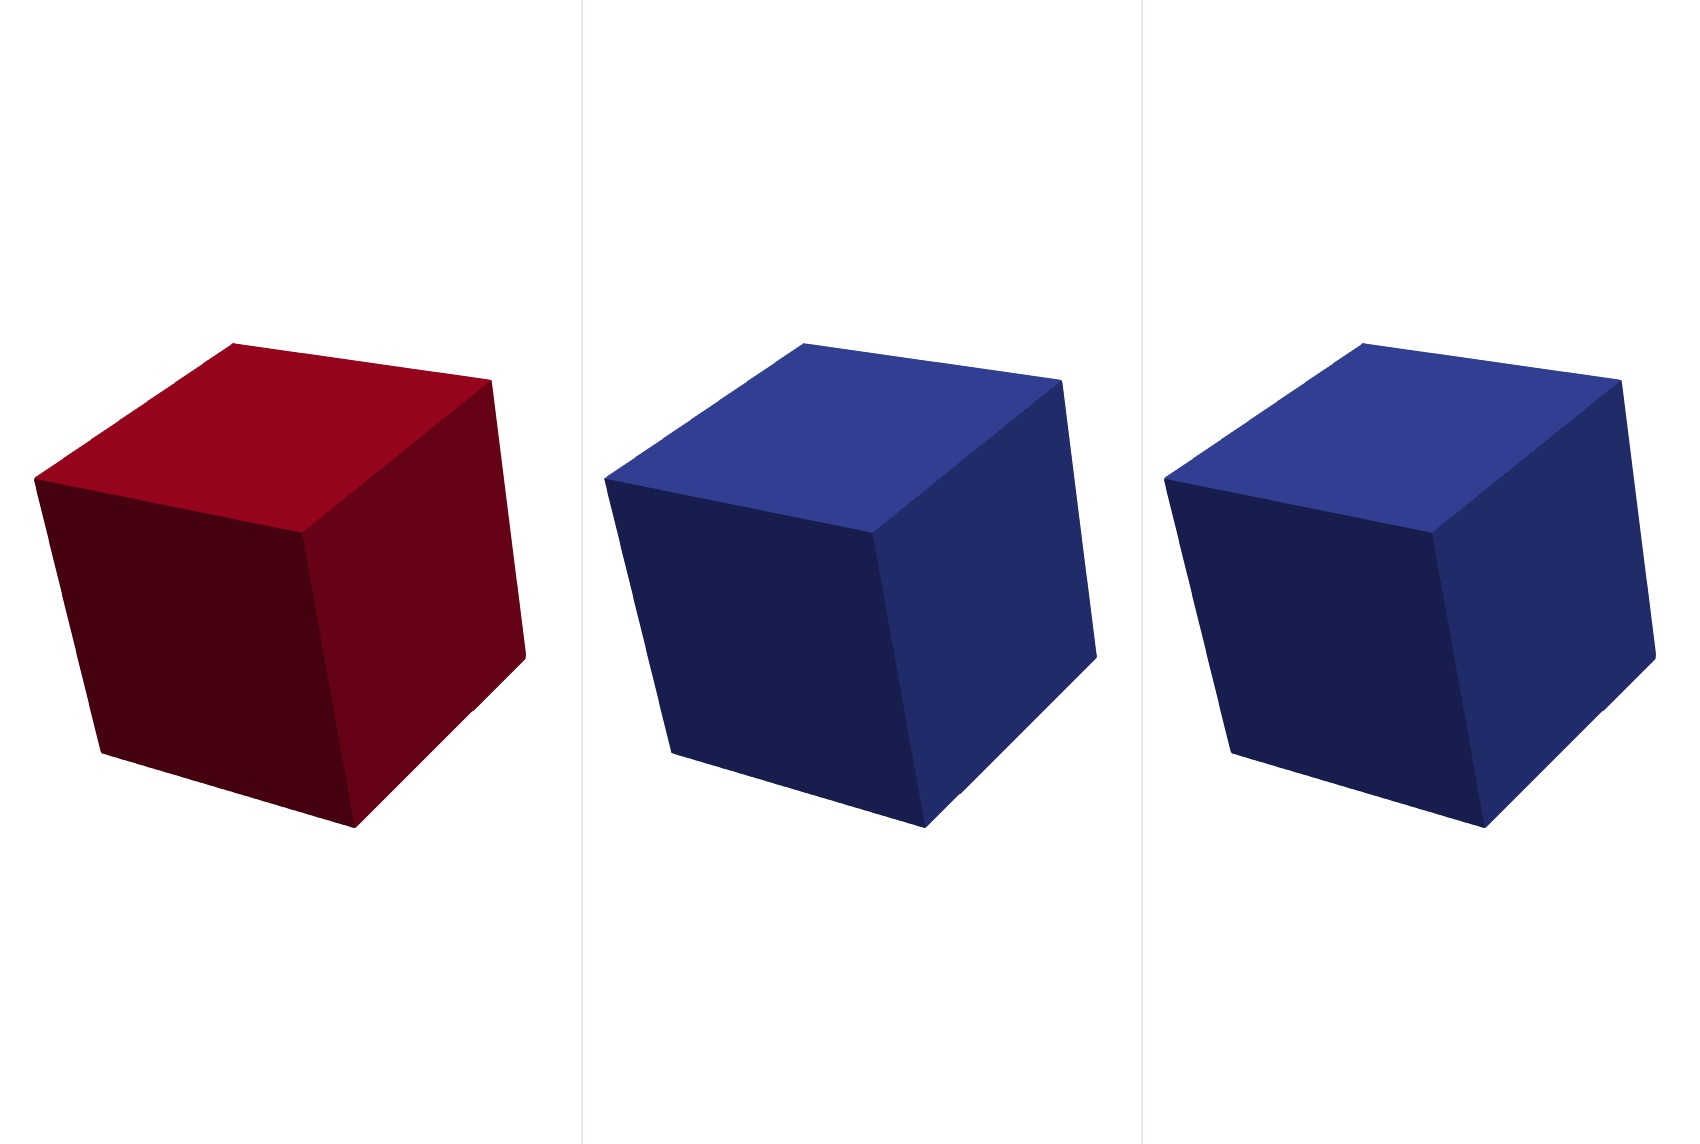
\includegraphics[width=0.32\textwidth]{img/basis/1.jpg}} & $\lo\begin{array}{c}0\\0\\y \end{array}\ro$ & \raisebox{-0.5\totalheight}{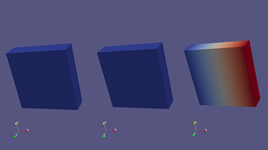
\includegraphics[width=0.32\textwidth]{img/basis/9.jpg}}\\
		\vspace{-2mm}
		$\lo\begin{array}{c}0\\1\\0 \end{array}\ro$ & \raisebox{-0.5\totalheight}{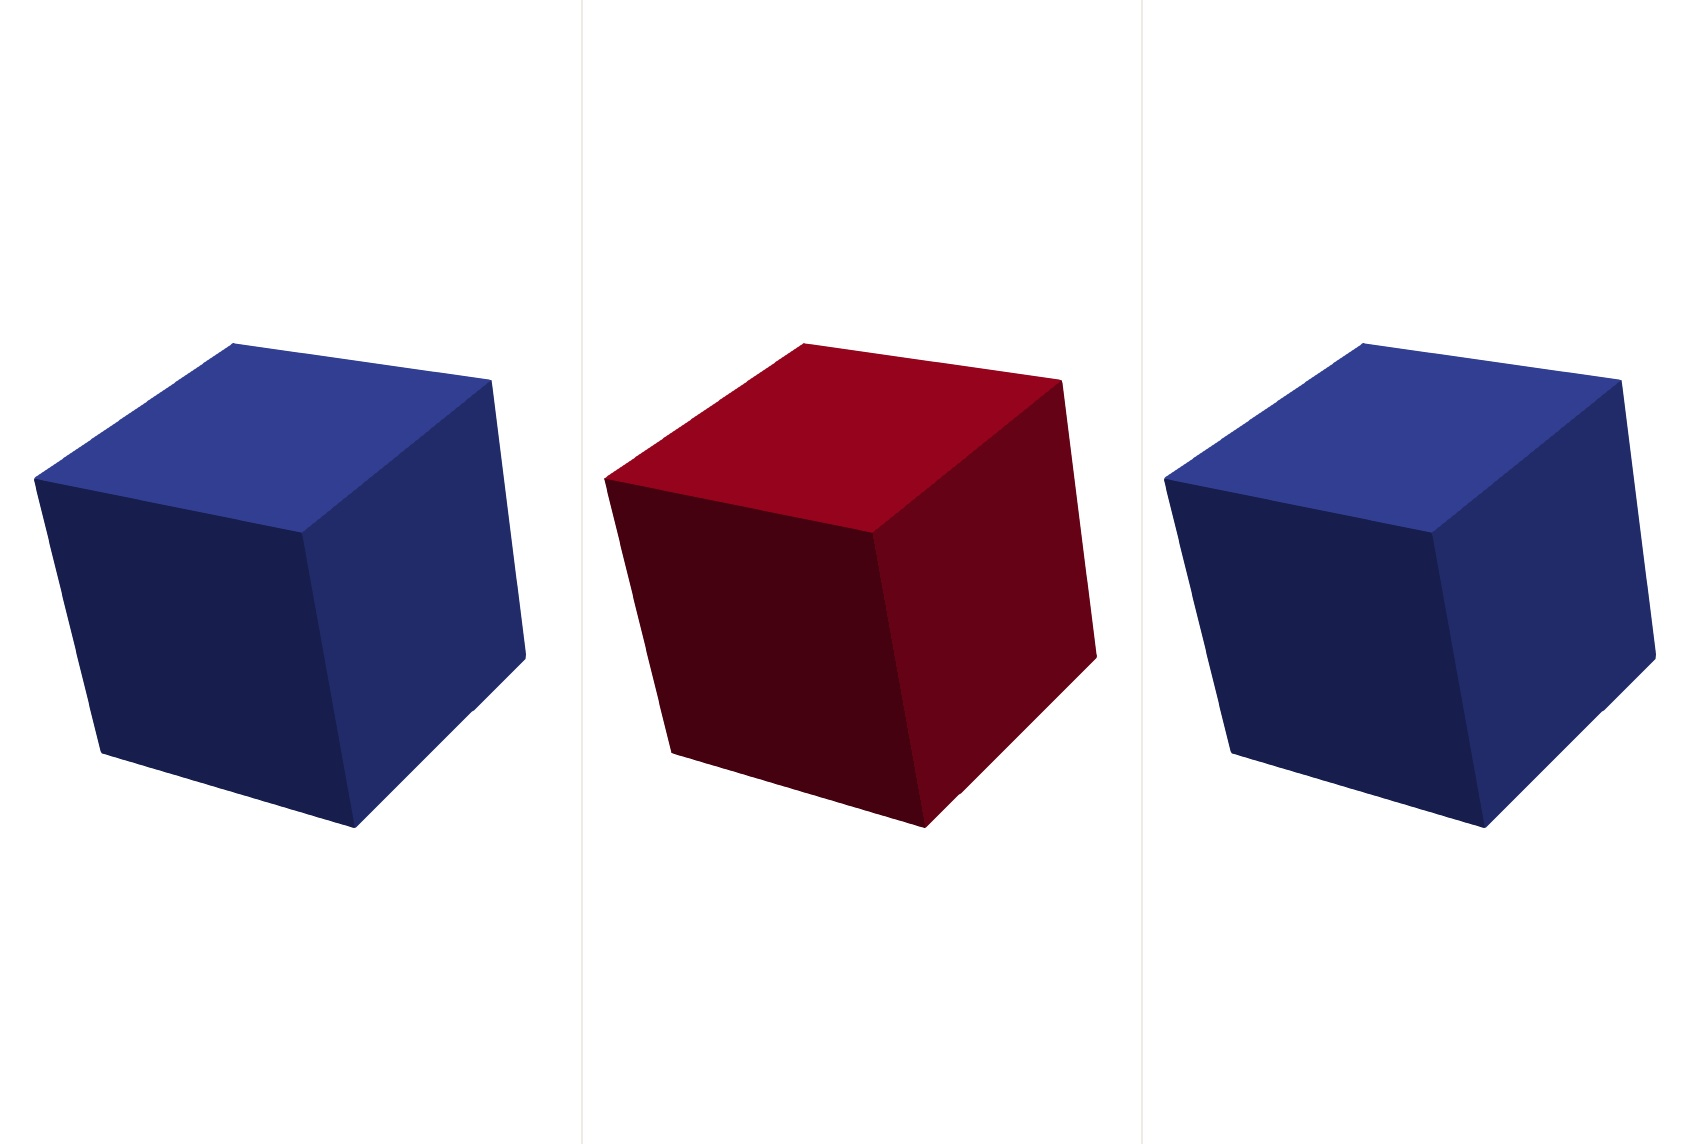
\includegraphics[width=0.32\textwidth]{img/basis/2.jpg}} & $\lo\begin{array}{c}z\\0\\0 \end{array}\ro$ & \raisebox{-0.5\totalheight}{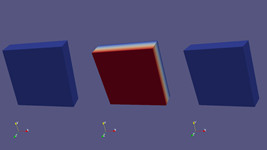
\includegraphics[width=0.32\textwidth]{img/basis/5.jpg}}\\
		\vspace{-2mm}
		$\lo\begin{array}{c}0\\0\\1 \end{array}\ro$ & \raisebox{-0.5\totalheight}{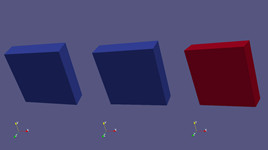
\includegraphics[width=0.32\textwidth]{img/basis/3.jpg}} & $\lo\begin{array}{c}0\\z\\0 \end{array}\ro$ & \raisebox{-0.5\totalheight}{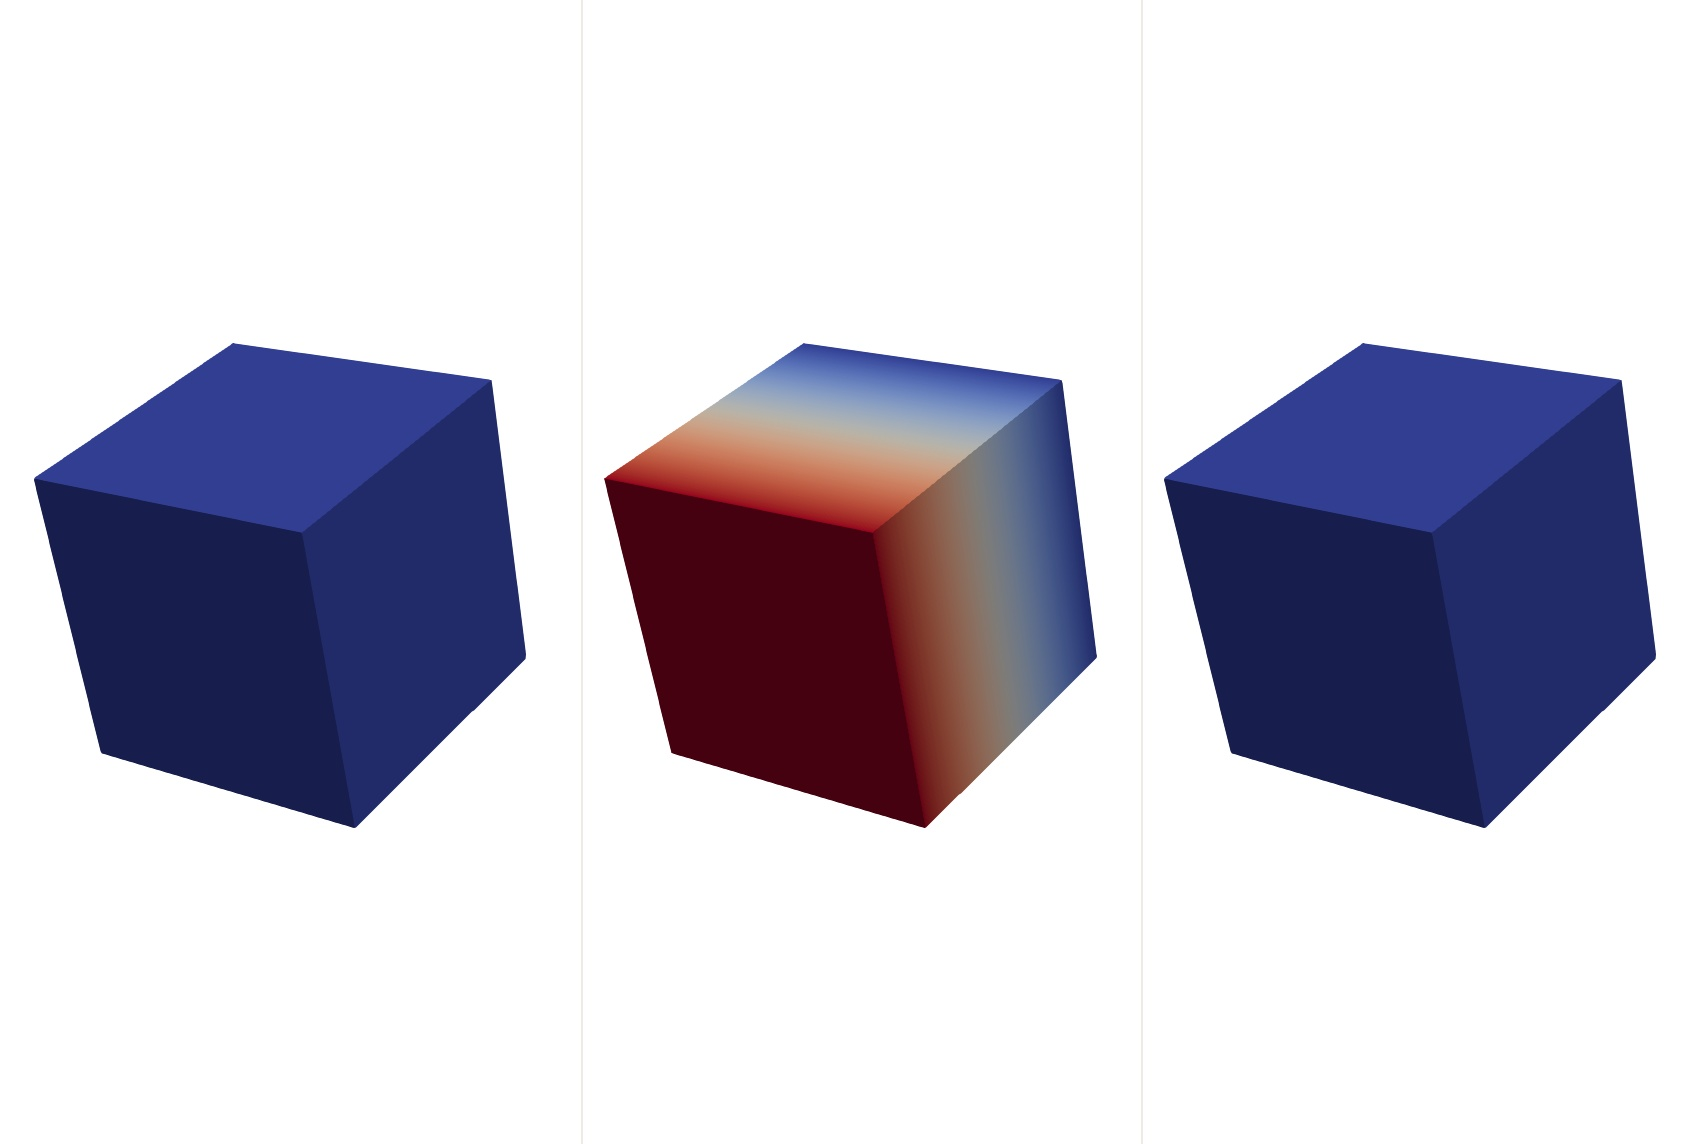
\includegraphics[width=0.32\textwidth]{img/basis/7.jpg}}\\
			\vspace{-2mm}
		$\lo\begin{array}{c}y\\0\\0 \end{array}\ro$ & \raisebox{-0.5\totalheight}{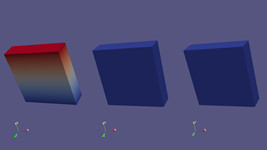
\includegraphics[width=0.32\textwidth]{img/basis/4.jpg}} & $\lo\begin{array}{c}0\\0\\x \end{array}\ro$ & \raisebox{-0.5\totalheight}{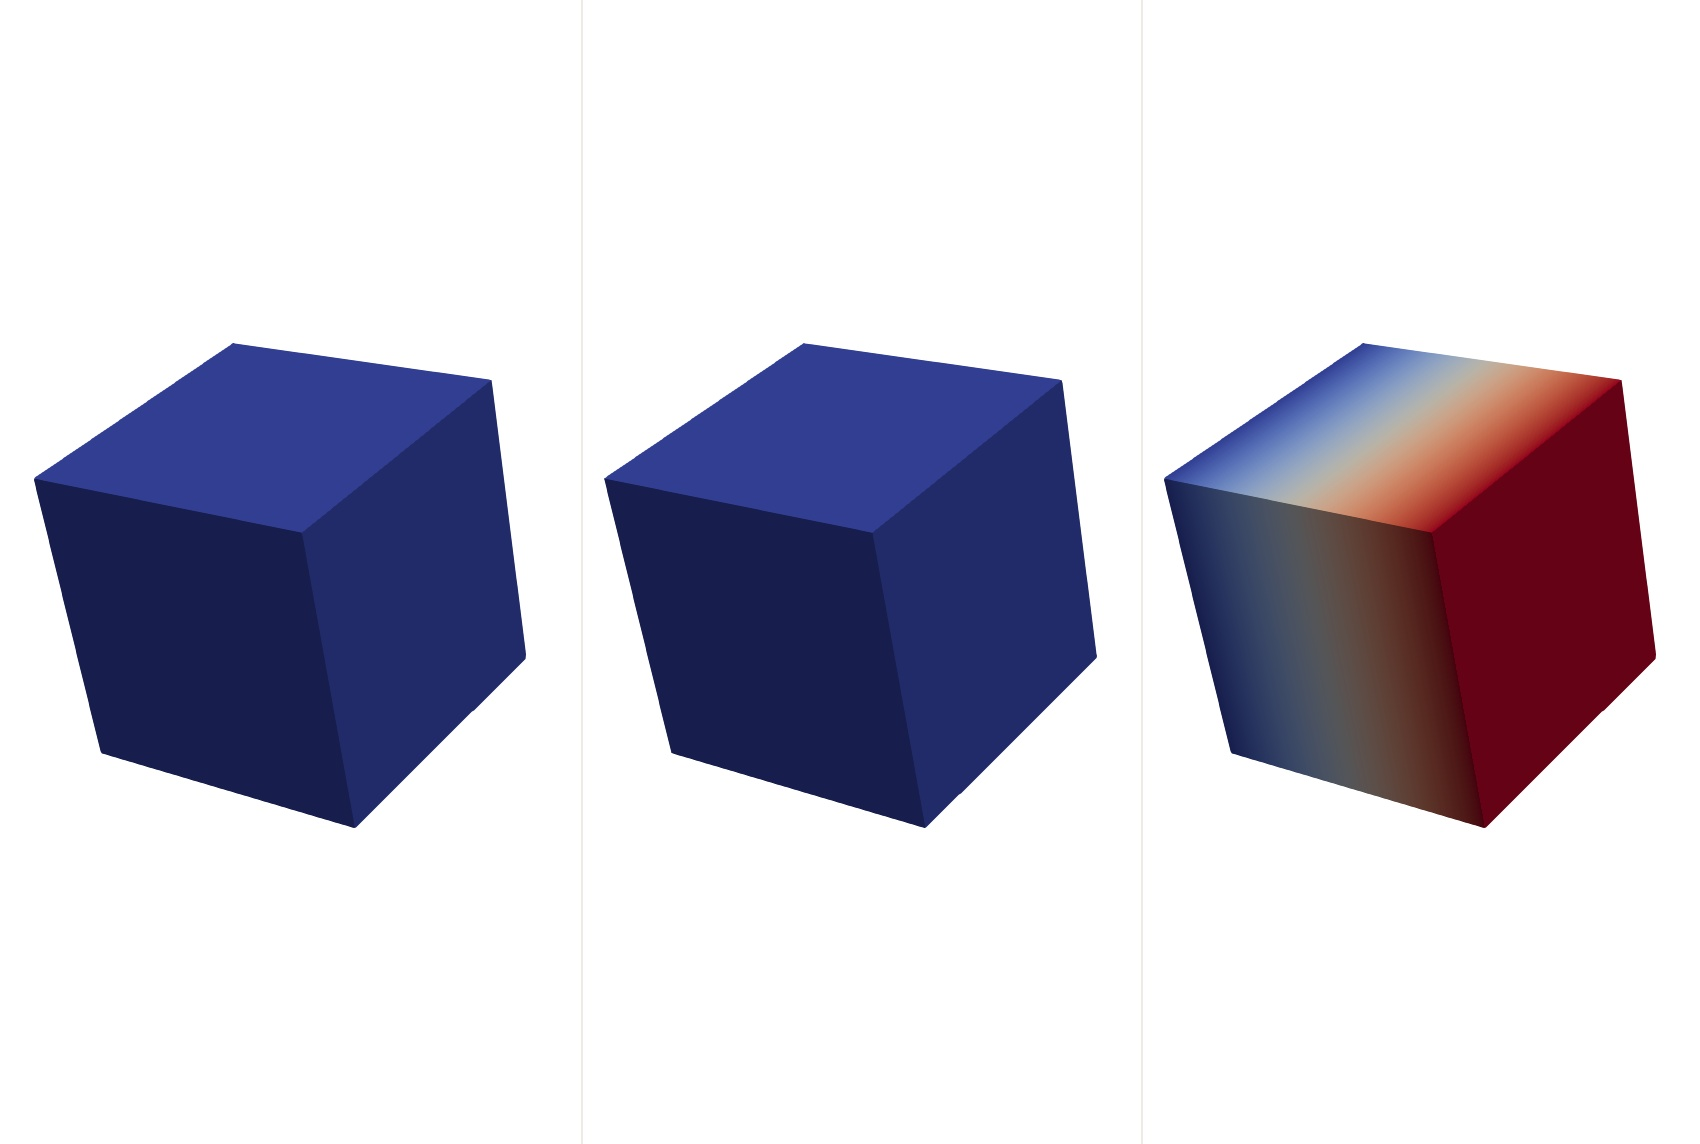
\includegraphics[width=0.32\textwidth]{img/basis/8.jpg}}\\
			\vspace{-2mm}
		$\lo\begin{array}{c}0\\x\\0 \end{array}\ro$ & \raisebox{-0.5\totalheight}{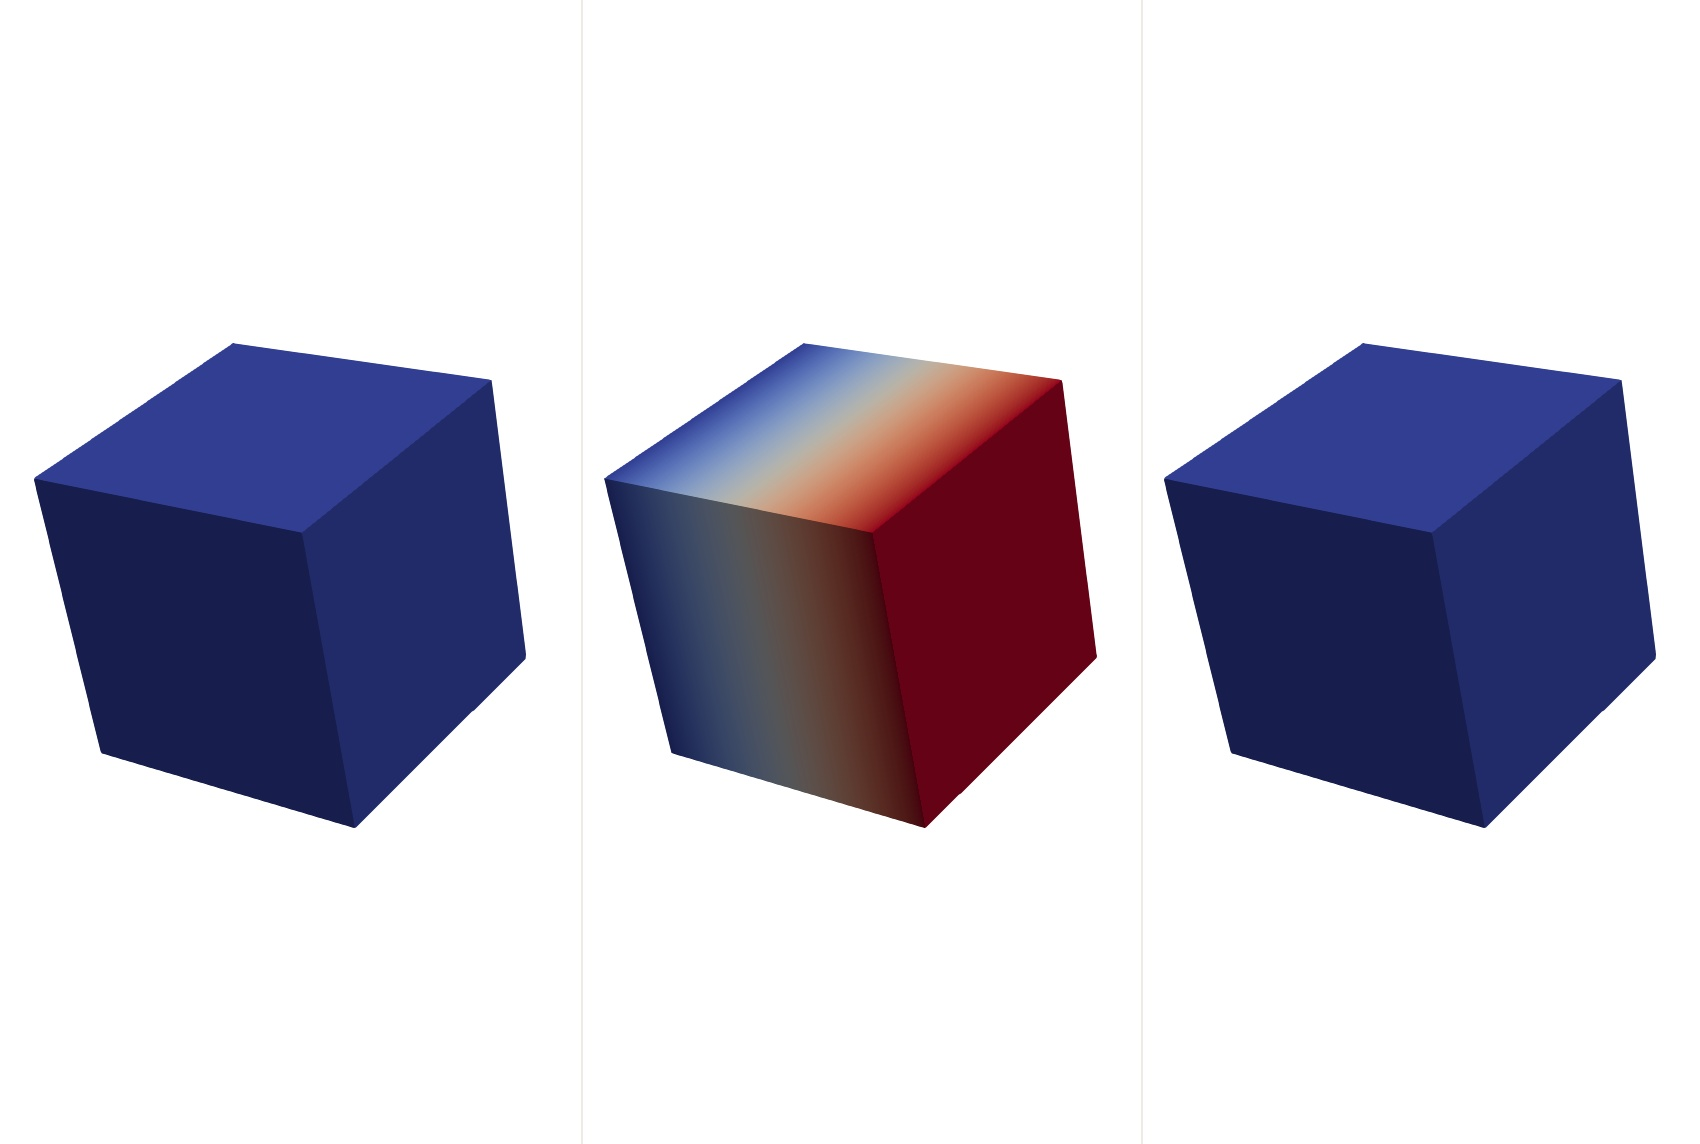
\includegraphics[width=0.32\textwidth]{img/basis/6.jpg}} & $\lo\begin{array}{c}x\\-y\\0 \end{array}\ro$ & \raisebox{-0.5\totalheight}{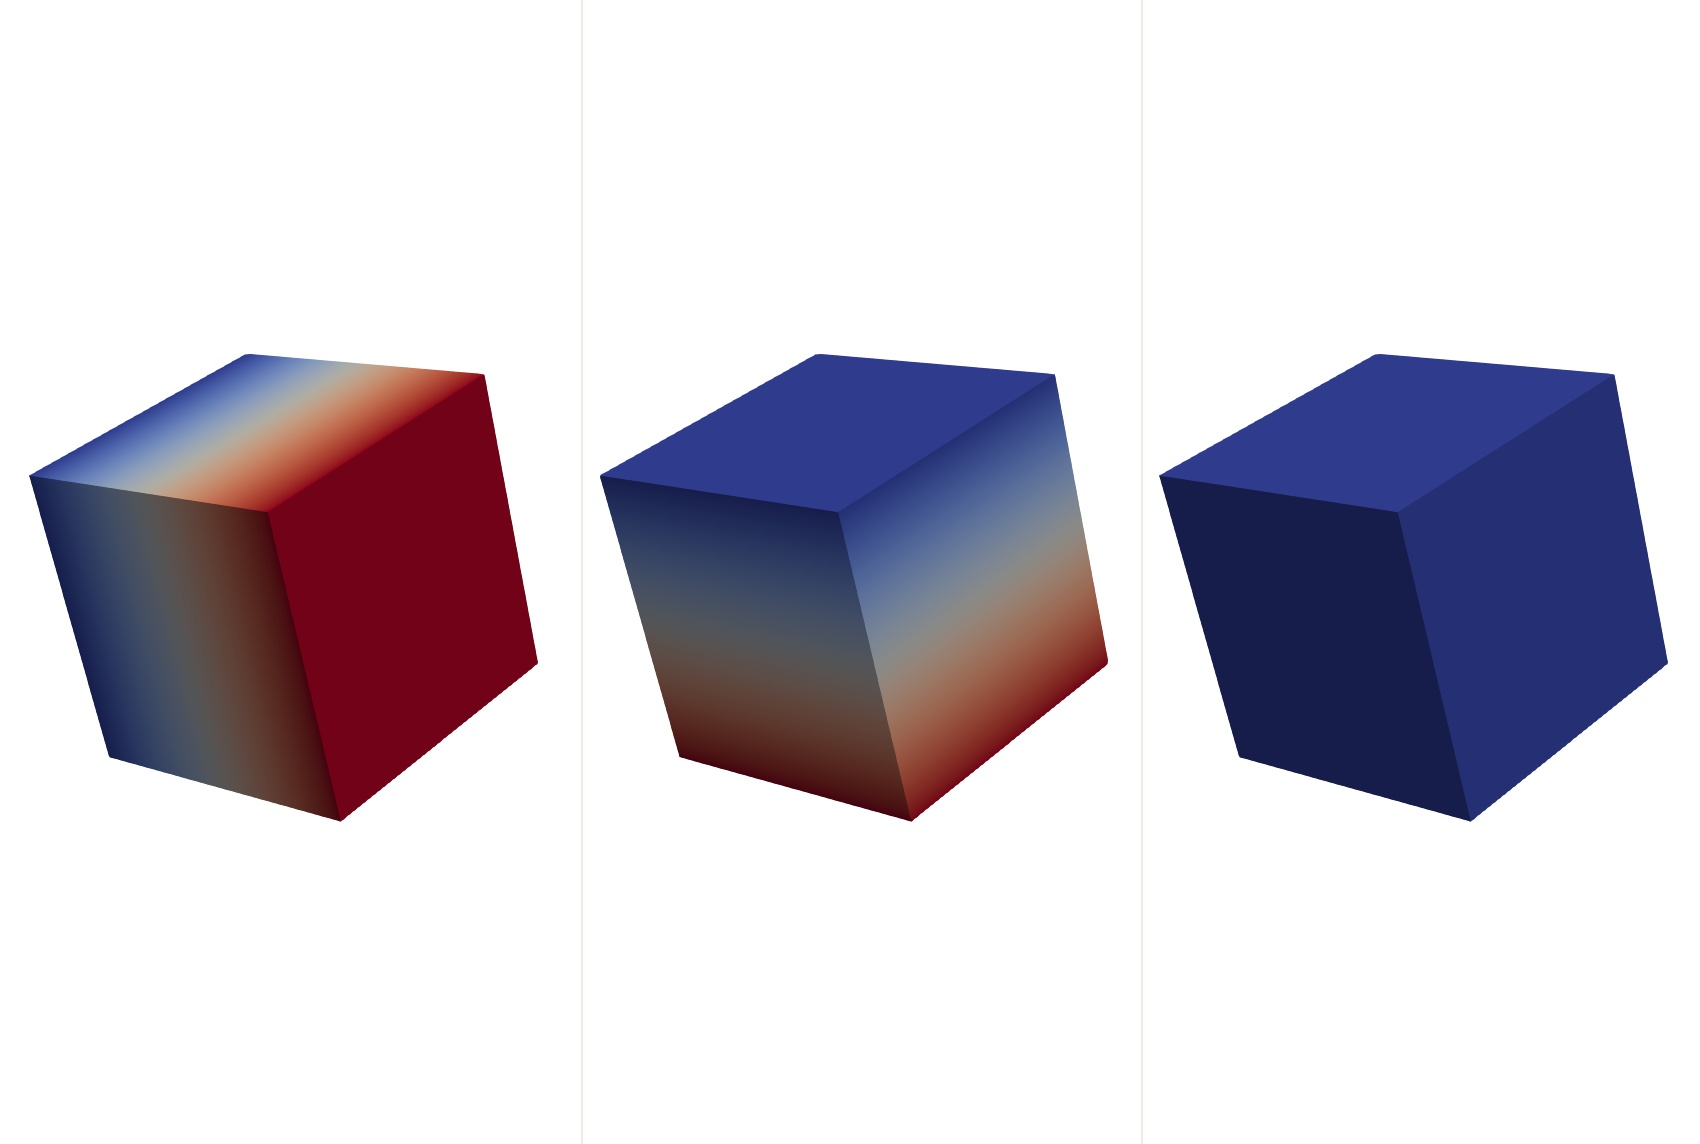
\includegraphics[width=0.32\textwidth]{img/basis/10.jpg}}\\	
			\vspace{-2mm}
		$\lo\begin{array}{c}x\\0\\-z \end{array}\ro$ & \raisebox{-0.5\totalheight}{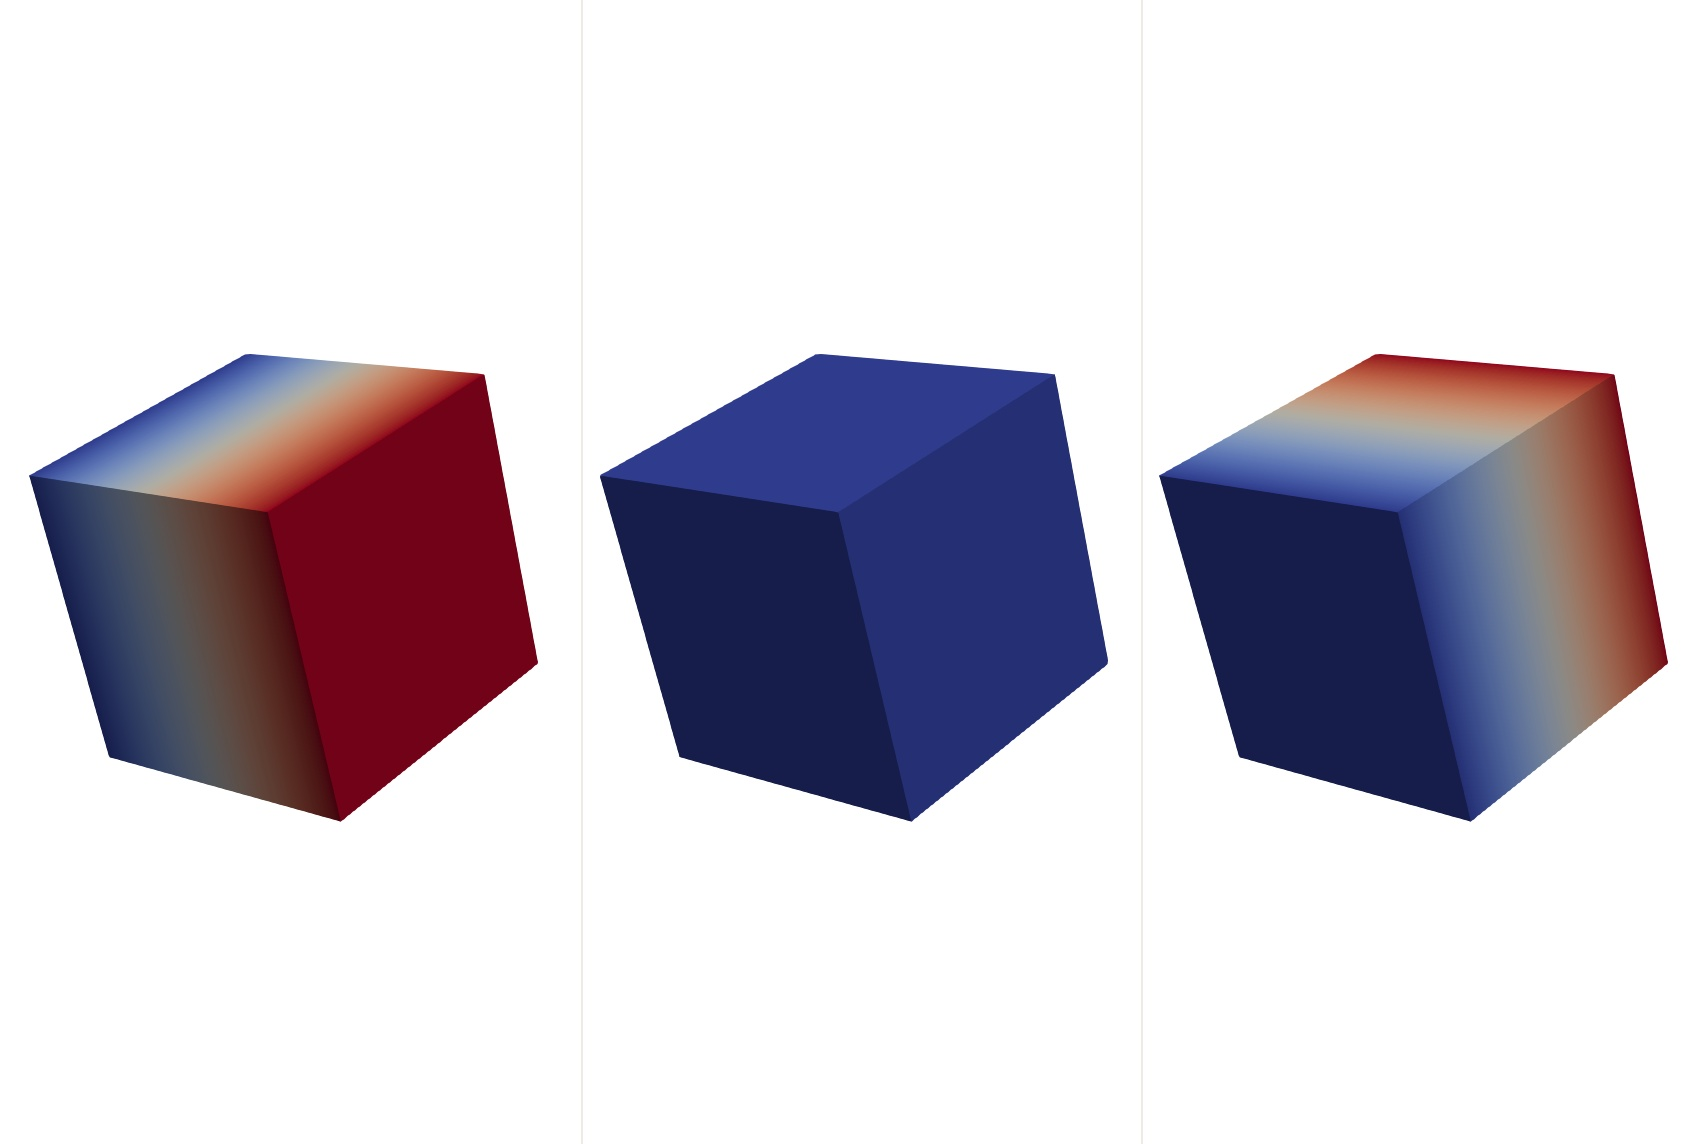
\includegraphics[width=0.32\textwidth]{img/basis/11.jpg}}
		\\	
			\hline		
		\end{tabular*}
		\caption{Divergence-free space basis}
	\label{tbl:divFreeBasis}
\end{table}
In \cref{tbl:divFreeBasis}, it is obvious that only one function actually has more nonzero components.
\paragraph{}
In what follows, the notation $\left[V_h\right]^8$ used before will be used for the space where the last three components are replaced by $V_h^B$. Note that there are some technicalities with respect to the usage of $V_h^B$ needed to be handled in computation, e.g. in \cref{vertexBasedAlpha}, or later in \cref{Final_Integration_Fn,Final_Integration_Fn_b} that we do not explicitly attend to.